\section{Die transzendente Erweiterung}
Sei $L\mid K$ eine Körpererweiterung.
\begin{definition}[algebraisch abhängig]
	\begin{enumerate}[label=(\alph*)]
		\item $a_1$, $\dots$, $a_n \in L$ sind \begriff{algebraisch abhängig} über $K$, wenn ein $0 \neq f \in K(X_1,\dots, X_n)$ existiert mit  $f(a_1, \dots, a_n) = 0$.
		\item $(a_i)_{i\in I}$ ist \begriff{algebraisch abhängig} über $K$, wenn ein endliches $J \subseteq I$ existiert und $(a_i)_{i\in J}$ ist algebraisch abhängig über $K$.
	\end{enumerate}
\end{definition}
\begin{*example}[nicht aus VL, sondern ergänzt!]
	Betrachte die reellen Zahlen $\sqrt{\pi} \und 2\pi +1$, beide sind transzendent über $\Q$. Die Singletons $\set{\sqrt{\pi}}\und \set{2\pi +1}$ sind algebraisch unabhängig über $\Q$. Aber die Vereinigung $\set{\sqrt{\pi}, 2\pi +1}$ ist nicht algebraisch unabhängig in $\Q$, da
	\begin{align*}
		P(x,y) = 2x^2 - y + 1 = 0
	\end{align*}
	ist, wenn $x = \sqrt{\pi} \und y = 2\pi +1$ gesetzt sind.
\end{*example}
\begin{remark}
	\begin{enumerate}[label=(\alph*)]
		\item $(a)$ ist algebraisch abhängig über $K \iff a$ ist algebraisch über $K$
		\item $L = K(X_1,\dots, X_n) = \Quot(K[X_1,\dots, X_n])$ $\implies$ $X_1$, $\dots$, $X_n$ sind algebraisch unabhängig über $K$
		\item Sind $\pi$, $e$ unabhängig über $\Q$?	Falls ``Ja'', wäre z.B. $\pi+e$ transzendent über $\Q$
	\end{enumerate}
\end{remark}
\begin{definition}[rein transzendent]
	$L \mid K$ \begriff{rein transzendent} $:\!\!\iff L = K(\Halb) \mit \Halb = (a_i)_{i\in I}$ algebraisch unabhängig über $K$.
\end{definition}
\begin{lemma}
	\proplbl{1_5_4}
	$\Halb = (a_i)_{i \in I}$ algebraisch unabhängig über $K \implies K(\Halb) \cong_K K(X_i \colon i \in I) = \Quot(K[X_i \colon i \in I])$. 
\end{lemma}
\begin{proof}
	Betrachte $K$-Isomorphismus
	\begin{flalign*}
		\qquad&\varphi = \left\lbrace\begin{array}{@{}l@{\;}l}
			K[X_i \colon I \in I] &\to K[a_i : i \in I]\\
			f & \mapsto f(\Halb)
		\end{array}\right. &
	\end{flalign*}
	Da $\Halb$ algebraisch unabhängig über $K$, ist $\Ker(\varphi) = (0)$\\
	$\implies K(\Halb) = \Quot(K[\Halb]) \cong_K \Quot(K[X_i : i \in I])$.
\end{proof}
\begin{proposition}
	$L\mid K$ rein transzendent $\implies \tilde{K} = K$.
\end{proposition}
\begin{proof}
	Nach \propref{1_5_4} sei o.E. $L = K(X_i : i \in I)$. Weiter o. E. $I = \set{1, \dots,n}$ endlich. Sei $\alpha \in L$ algebraisch über $K$. Definiere $f = \MinPol(\alpha \mid K)$.\\
	$f$ irreduzibel in $K[X] \xRightarrow{\text{\person{Gauss}}} f$ irreduzibel in $K[X_1, \dots, X_n][X]$
	\begin{itemize}[topsep=-2pt]
	\item[$\xRightarrow{\text{\person{Gauss}}}$] $f$ irreduzibel in $K(X_1, \dots, X_n)[X]$
	\item[$\xRightarrow{\alpha\in L}$] $\deg(f) = 1$
	\item[$\implies$] $\alpha \in K$
	\end{itemize}
\end{proof}
\begin{remark}
	Die Umkehrung gilt nicht, da z.B. $L = \C$. Sei $K = \tilde{\Q}$, dann $\tilde{K} = K$, aber $L\mid K$ nicht rein transzendent. Ist $L = K[\Halb]$, $\Halb = (a_i)_{i\in I}$ algebraisch unabhängig, so wäre $a_i \in L$ aber $\sqrt{a_i} \in \bar{L}\setminus L$.
\end{remark}
\begin{definition}[Transzendentbasis]
	$\Halb = (a_i)_{i\in I}$ ist eine \begriff{Transzendentbasis} von $L \mid K$ $:\!\! \iff$ $\Halb$ ist algebraisch unabhängig über $K$ und $L\mid K(\Halb)$ algebraisch.
\end{definition}
\begin{lemma}
	\proplbl{1_5_8}
	$\Halb = (a_i)_{i \in I} \subseteq L$ ist genau dann eine Transzendentbasis von $L \mid K$, wenn $\Halb$ maximal algebraisch unabhängig über $K$ ist.
\end{lemma}
\begin{proof}\leavevmode\vspace*{\dimexpr-\baselineskip+2\lineskip}
	\begin{itemize}
		\item[($\Leftarrow$)] $a \in L \setminus K(\Halb) \xRightarrow{\text{maximal}} \Halb \cup \set{a}$ algebraisch abhängig, d.h. existieren $i_1$, $\dots$, $i_n \in I$, $0 \neq f \in K[X_1, \dots, X_n, X]$ mit $f(a_{i_1}, \dots, a_{i_n}, a) = 0$
		
		$a_{i_1}$, $\dots$, $a_{i_n}$ algebraisch unabhängig über $K$\\
		$\implies \underbrace{f(a_{i_1}, \dots, a_{i_n}, X)}_{\in K(a_{i_1}, \dots, a_{i_n})[X]\subseteq K(\Halb)[X]}\neq 0$\\
		$\implies a$ ist algebraisch über $K(\Halb)$
		\item[($\Rightarrow$)] $a \in L\setminus K(\Halb) \xRightarrow{L \setminus K(\Halb) \text{ alg.}}$ existiert $0 \neq f \in K(\Halb)[X] \mit f(a) = 0$\\
		O.E. (Problem: Nenner kann Koeffizienten in $K(\Halb)$ haben $\to$ Multiplikation mit Nenner, weil $f(a) =0$) $f \in K[\Halb][X]$, d.h. es existiert $g \in K[X_1, \dots, X_n][X]$ und $i_1,\dots, i_n \in I \mit f(X) = g(a_{i_1},\dots, a_{i_n}, X)$ und $\Halb \cup \set{a}$ ist algebraisch abhängig.
	\end{itemize}
\end{proof}
\begin{proposition}
	Es gibt eine Transzendenzbasis von $L\mid K$.
\end{proposition}
\begin{proof}
	Nach Lemma von \person{Zorn} gibt es eine Familie $\Halb$ in $L$, die maximal algebraisch unabhängig über $K$ ist.
\end{proof}
\begin{conclusion}
	Jede Erweiterung $L\mid K$ lässt sich zerlegen als
\begin{center} % tikzcd was bitchy, compiled and included the pdf.
	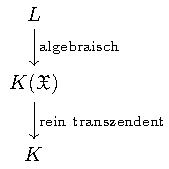
\includegraphics{./tikz/lemma_1_5_10.pdf}
\end{center}
\end{conclusion}
\begin{lemma}
	\proplbl{1_5_11}
	Ist $\caly = (b_j)_{j \in J}$ mit $L\mid K(\caly)$ algebraisch und $\Halb = (a_i)_{i\in I}$ algebraisch unabhängig über $K$, so existiert $J_0 \subseteq J$ mit $\Halb \cup (b_j)_{j \in J_0}$ eine Transzendenzbasis von $L \mid K$.
\end{lemma}
\begin{proof}
	Nach dem Lemma von \person{Zorn} existiert $J_0 \subseteq J$ maximal mit $\Halb' = \Halb \cup (b_j)_{j \in J_0}$ algebraisch unabhängig über $K$. Für jedes $j \in J$ ist $\Halb' \cup \set{b_j}$ algebraisch abhängig über $K$, somit $b_j$ algebraisch über $K(\Halb')$\\
	 $\implies K(\Halb \cup \caly) \mid K(\Halb')$ algebraisch\\
	$L \mid K(\caly)$ algebraisch $\implies L\mid K(\Halb \cup \caly)$ algebraisch $\xRightarrow{\text{alg. transitiv}} L \mid K(\Halb')$ algebraisch. Somit ist $\Halb'$ eine Transzendenzbasis.
\end{proof}
\begin{theorem}[Steinitz, 1910]
	Je zwei Transzendenzbasen von $L \mid K$ besitzen die gleiche Mächtigkeit.
\end{theorem}
\begin{proof}
	Seien $\Halb = (a_i)_{i\in I}$, $\caly = (b_j)_{j \in J}$ Transzendenzbasis von $L \mid K$.\\ 
	Beweisen hier nur für $J$ endlich:\\
	Wegen Symmetrie genügt es zu zeigen, dass $\abs{I} \le \abs{J}$.\\
	Induktion nach $n = \abs{J}$:
	\begin{itemize}[topsep=-6pt,left=3em,itemsep=\lineskip,parsep=\lineskip]
		\item[$n =0$:] $L \mid K$ algebraisch $\implies \abs{I} = 0$
		\item[$n > 0$:] $L \mid K$ nicht algebraisch $\implies \abs{I} > 0$. %TODO
		
		O.E. $1\in I$. Nach \propref{1_5_11} existiert ein $J_0\subset J$ mit $\{a_i\}\cup (b_j)_{j\in J_0}$ eine Transzendentenbasis von $L\mid K$. Da $\mathcal Y$ maximal algebraisch unabhängig über $K$ ist, ist $\vert J_0\vert \le \vert J\vert - 1$.
		
		Sowohl $\Halb' = (a_i)_{i\in I\setminus\{1\}}$ als auch $(b_j)_{j\in J_0}$ sind Transzendentenbasen von $L\mid K(a_1)$:
		\begin{adjustwidth}{0.75em}{-6pt}
		$K(a_1)(\Halb') = K(\Halb)$ $\Rightarrow$ $L\mid K(a_1)(\Halb')$ algebraisch, analog $L\mid K(a_1)(b_j)_{j\in J_0}$ algebraisch.
		
		Wäre $\Halb'$ algebraisch abhängig über $K(a_1)$, so existierte ein \begin{flalign*}\qquad&0\neq f\in K(a_1)[X_1,\dots, X_m],\quad i_1, \dots, i_m\in I\setminus\{1\} &
		\end{flalign*}
		mit $f(a_{i_1},\dots,a_{i_m}) = 0$.\\
		O.E. ist $f\in K[a_1][X_1,\dots,X_m]$, d.h. es existiert $g\in K[X,X_1,\dots, X_m]$ mit
		\begin{flalign*}
			\qquad& f(X_1,\dots,X_m) = g(a_1,X_1,\dots,X_m) &
		\end{flalign*}
		im Widerspruch zur algebraischen Unabhängigkeit von $\Halb$.
		\end{adjustwidth}
		
		$\xRightarrow{\text{(IH)}}$ $\vert I\vert -1 \le \vert J_0\vert$
		$\Rightarrow$ $\vert I\vert -1\le \vert J\vert -1$ $\Rightarrow$ $\vert I \vert\le \vert J\vert$.
	\end{itemize}
\end{proof}
\begin{definition}[Transzendenzgrad]
	Der \begriff{Transzendenzgrad} von $L \mid K$ ist die Mächtigkeit $\transdeg(L\mid K)$ einer Tarnszendenzbasis von $L \mid K$.
\end{definition}
\begin{conclusion}
	Sind $L \subseteq L \subseteq M$ Körper, so ist
	\begin{flalign*}
		\qquad&\transdeg(M\mid K) = \transdeg(M \mid L) + \transdeg(L \mid K).&
	\end{flalign*}
\end{conclusion}
\vspace*{-3pt}
\begin{proof}
	Ist $\Halb$ eine Transzendentenbasis von $L\mid K$, $\mathcal Y$ eine Transzendentenbasis von $M\mid L$, so ist $\Halb\cup\mathcal Y$ eine Transzendentenbasis von $M\mid K$.
	
	\begin{itemize}[topsep=-7pt,parsep=\lineskip,itemsep=\lineskip]
		\item $\Halb\cup\mathcal Y$ ist algebraisch unabhängig über $K$. Denn ist $f(a_{i_1},\dots,a_{i_n},b_{j_1},\dots,b_{j_m}) = 0$ mit $i_1$, $\dots$, $i_n\in I$ und $j_1$, $\dots$, $j_m\in J$ sowie $0\neq f\in K[X_1,\dots,X_n,Y_1,\dots,Y_m]$, so gälte:
		\begin{itemize}[topsep=-3pt]
			\item $f\in K[X_1,\dots,X_n]$: im Widerspruch zur algebraischen Unabhängigkeit von $\Halb$ über $K$
			\item $f\notin K[X_1,\dots,X_n]$: $0\neq f(a_{i_1},\dots,a_{i_n}, Y_1,\dots,Y_{m})\in L[Y_1,\dots,Y_m]$ im Widerspruch zur algebraischen Unabhängigkeit von $\mathcal Y$ über $L$.
		\end{itemize}
		\vspace*{-1pt}
		\item $M\mid K(\Halb\cup\mathcal Y)$ algebraisch:
		\begin{itemize}[topsep=-5pt,left=5em,parsep=\lineskip,itemsep=\lineskip]
			\item[] $L(\mathcal Y) = K(\Halb\cup \mathcal Y)(L)$
			\item[$\xRightarrow{L\mid K(\Halb)\;\text{alg.}}$] $L(\mathcal Y)\mid K(\Halb\cup \mathcal Y)$ algebraisch
			\item[$\Rightarrow$] $M\mid K(\Halb\cup\mathcal Y)$ algebraisch.
		\end{itemize}
	\end{itemize}
\end{proof}